\documentclass[letterpaper,12pt,fleqn]{article}
\usepackage{matharticle}
\usepackage{tikz}
\usetikzlibrary{positioning}
\pagestyle{plain}
\begin{document}
Cavallaro, Jeffery \\
Math 275A \\
Homework \#1

\bigskip

\begin{theorem}[Exercise 1.3]
  For a function \(f:X\to Y\) and sets \(A,B\subset Y\):
  \begin{itemize}
  \item \(f^{-1}(A\cup B)=f^{-1}(A)\cup f^{-1}(B)\)
  \item \(f^{-1}(A\cap B)=f^{-1}(A)\cap f^{-1}(B)\)
  \end{itemize}
\end{theorem}

\begin{proof}
  \begin{align*}
    x\in f^{-1}(A\cup B) &\iff f(x)\in A\cup B \\
    &\iff f(x)\in A\ \text{or}\ f(x)\in B \\
    &\iff x\in f^{-1}(A)\ \text{or}\ x\in f^{-1}(B) \\
    &\iff x\in f^{-1}(A)\cup f^{-1}(B)
  \end{align*}
  Therefore, \(f^{-1}(A\cup B)=f^{-1}(A)\cup f^{-1}(B)\).
  \begin{align*}
    x\in f^{-1}(A\cap B) &\iff f(x)\in A\cap B \\
    &\iff f(x)\in A\ \text{and}\ f(x)\in B \\
    &\iff x\in f^{-1}(A)\ \text{and}\ x\in f^{-1}(B) \\
    &\iff x\in f^{-1}(A)\cap f^{-1}(B)
  \end{align*}
  Therefore, \(f^{-1}(A\cap B)=f^{-1}(A)\cap f^{-1}(B)\).
\end{proof}

\begin{theorem}[Restatement of 1.8]
  Let \(A\) and \(B\) be sets such that \(A\subset B\).  If \(B\) is countable then \(A\) is countable.
\end{theorem}

\begin{lemma}
  Let \(\set{U_i:i\in N}\) be a countably infinite number of countably infinite sets such that the \(U_i\) are
  pairwise disjoint.  Then:
  \[U=\bigcup_{i\in\N}U_i\]
  is countable.
\end{lemma}

\begin{proof}
  Let \(U_i=\set{u_{ij}:j\in\N}\) and arrange the \(U_i\) as the rows of a matrix.  Note that the \(u_{ij}\) are
  distinct and in one-to-one correspondence with the elements of \(U\).

  Now, enumerate the \(u_{ij}\) along the diagonals as follows:

  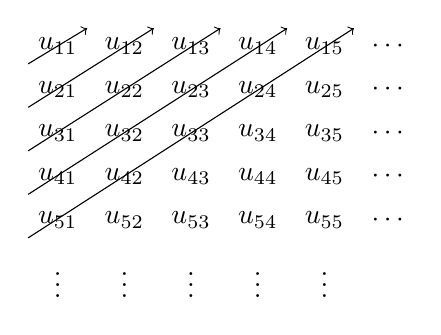
\begin{tikzpicture}[node distance=0.1cm]
    \node (u11) at (0,0) {\(u_{11}\)};
    \node (u12) [right=of u11] {\(u_{12}\)};
    \node (u13) [right=of u12] {\(u_{13}\)};
    \node (u14) [right=of u13] {\(u_{14}\)};
    \node (u15) [right=of u14] {\(u_{15}\)};
    \node (u1n) [right=of u15] {\(\cdots\)};
    \node (u21) [below=of u11] {\(u_{21}\)};
    \node (u22) [below=of u12] {\(u_{22}\)};
    \node (u23) [below=of u13] {\(u_{23}\)};
    \node (u24) [below=of u14] {\(u_{24}\)};
    \node (u25) [below=of u15] {\(u_{25}\)};
    \node (u2n) [right=of u25] {\(\cdots\)};
    \node (u31) [below=of u21] {\(u_{31}\)};
    \node (u32) [below=of u22] {\(u_{32}\)};
    \node (u33) [below=of u23] {\(u_{33}\)};
    \node (u34) [below=of u24] {\(u_{34}\)};
    \node (u35) [below=of u25] {\(u_{35}\)};
    \node (u3n) [right=of u35] {\(\cdots\)};
    \node (u41) [below=of u31] {\(u_{41}\)};
    \node (u42) [below=of u32] {\(u_{42}\)};
    \node (u43) [below=of u33] {\(u_{43}\)};
    \node (u44) [below=of u34] {\(u_{44}\)};
    \node (u45) [below=of u35] {\(u_{45}\)};
    \node (u4n) [right=of u45] {\(\cdots\)};
    \node (u51) [below=of u41] {\(u_{51}\)};
    \node (u52) [below=of u42] {\(u_{52}\)};
    \node (u53) [below=of u43] {\(u_{53}\)};
    \node (u54) [below=of u44] {\(u_{54}\)};
    \node (u55) [below=of u45] {\(u_{55}\)};
    \node (u5n) [right=of u55] {\(\cdots\)};
    \node (um1) [below=of u51] {\(\vdots\)};
    \node (um2) [below=of u52] {\(\vdots\)};
    \node (um3) [below=of u53] {\(\vdots\)};
    \node (um4) [below=of u54] {\(\vdots\)};
    \node (um5) [below=of u55] {\(\vdots\)};
    \draw [->] (u11.south west) -- (u11.north east);
    \draw [->] (u21.south west) -- (u12.north east);
    \draw [->] (u31.south west) -- (u13.north east);
    \draw [->] (u41.south west) -- (u14.north east);
    \draw [->] (u51.south west) -- (u15.north east);
  \end{tikzpicture}

  This is a one-to-one correspondence between the \(u_{ij}\) and \(\N\) and hence the \(u_{ij}\) are countable.

  Therefore, \(U\) is countable.
\end{proof}

\begin{theorem}[1.12]
  The union of countably many countable sets is countable.
\end{theorem}

\begin{proof}
  Let \(A=\bigcup_{i\in I}A_i\) be a union of countably many countable sets.  In order to remove duplicates from the
  \(A_i\) (elements in the intersections of two or more \(A_i\)), let:
  \begin{align*}
    A_1' &= A_1 \\
    A_i' &= A_i-\bigcup_{j=1}^{i-1}A_j
  \end{align*}
  Note that the \(A_i'\) are pairwise disjoint and \(A=\bigcup_{i\in I}A_i'\)

  Now arrange the \(A_i'\) as the rows of a matrix \(B\).  This means that the \(b_{ij}\) are distinct and in
  one-to-one correspondence with the elements of \(A\).  Let \(U\) be a matrix consisting of a countably infinite
  number of rows and columns as described in the preceding lemma.  There is an injection between the rows in \(B\)
  and the rows in \(U\).  Furthermore, there is an injection between the columns of each row \(B_i\) and its
  corresponding row \(U_i\).  Thus, there is a one-to-one correspondence between the elements of \(B\), and hence
  the elements of \(A\), and the elements of some subset \(C\) of the elements of \(U\).  But the subset of a
  countable set is countable (Theorem 1.8) and so \(C\) is countable.

  Therefore \(A\) is countable.
\end{proof}

\begin{theorem}[1.13]
  The set \(\Q\) is countable.
\end{theorem}

\begin{proof}
  Let \(\set{Q_i:i\in\N}\) be a family of sets where \(Q_i=\setb{\frac{p}{i}}{p\in\Z}\).  Note that:
  \[\Q=\bigcup_{i\in\N}Q_i\]
  But \(\set{Q_i:i\in\N}\) is a countable number of countable sets, and hence is countable (Theorem 1.2).

  Therefore, \(Q\) is countable.
\end{proof}

\begin{theorem}[1.16]
  The set of real numbers \(\R\) is uncountable.
\end{theorem}

\begin{proof}
  ABC that \((0,1)\) is countable.  This means that there exists some bijection \(f:\N\to(0,1)\).  Let \(a_{ij}\)
  be \(j^{th}\) decimal digit of the \(i^{th}\) number:
  \begin{align*}
    f(1) &= 0.a_{11}a_{12}a_{13}a_{14}a_{15}\cdots \\
    f(2) &= 0.a_{21}a_{22}a_{23}a_{24}a_{25}\cdots \\
    f(3) &= 0.a_{31}a_{32}a_{33}a_{34}a_{35}\cdots \\
    f(4) &= 0.a_{41}a_{42}a_{43}a_{44}a_{45}\cdots \\
    f(5) &= 0.a_{51}a_{52}a_{53}a_{54}a_{55}\cdots \\
    \vdots &= \vdots
  \end{align*}
  If \(f(n)\) is rational with more than one representation, for example: \(0.4\bar{9}=0.5\bar{0}\), then the
  repeating \(0\) case is selected.

  Now, let \(b=b_1b_2b_3b_4b_5\cdots\) where:
  \[b_i=\begin{cases}
  1, & a_{ii}\ne1 \\
  2, & a_{ii}=1
  \end{cases}\]
  So \(b\) never contains a \(0\) or \(9\) digit and thus the non-unique cases are avoided.  This means that
  \(b\in(0,1)\) but \(b\notin f(\N)\), contradicting the bijectiveness of \(f\).  Thus, \((0,1)\) is uncountable.
  But \((0,1)\subset\R\).

  Therefore, by the contrapositive of Theorem 1.8, \(\R\) is uncountable.
\end{proof}

\end{document}
